\documentclass[12pt,a4paper]{article}
\usepackage{color}
\usepackage{float}
\usepackage{graphicx}
\usepackage{indentfirst}
\usepackage{amsmath}
\usepackage{multirow}
\usepackage{url}
\usepackage{booktabs}
\def\degree{${}^{\circ}$}
\usepackage{amssymb}
\begin{document}

\vspace*{0.25cm}

\hrulefill

\thispagestyle{empty}

\begin{center}
\begin{large}
\sc{UM--SJTU Joint Institute \vspace{0.3em} \\ Introduction to Cryptography \\(VE475)}
\end{large}

\hrulefill

\vspace*{5cm}
\begin{Large}
\sc{{Project Report}}
\end{Large}

\vspace{2em}

\begin{large}
\sc{{Group 1\\
\vspace{0.5em}
bitcoin \\}}
\end{large}
\end{center}


\vfill

\begin{table}[h!]
\flushleft
\begin{tabular}{lll}
Name: Liu Niyiqiu \hspace*{2em}&
ID: 516370910118\hspace*{2em}
\\
Name: Xiang Zhiyuan \hspace*{2em}&
ID: 516370910118\hspace*{2em}
\\
Name: S \hspace*{2em}&
ID: 516370910118\hspace*{2em}
\\


\\

Date: 26 July 2019
\end{tabular}
\end{table}

\hfill

\newpage
\tableofcontents
\newpage

\section{Mining}
\subsection{Definition of Mining}
The bitcoin is a decentralized cryptocurrent. No authorities are present to authenticate each transaction. Thus the burden of verifying transactions and gathering valid transactions lies to the miners. The ultimate goal of a miner is to constitute a block by solving a mathematical problem, which will be described in the next section. To compensate the computational power spent by the miner, some bitcoins are given to the first miner that create a new block. Also, the payer in a transaction may specify a transaction fee that will be given to the miner. 
\subsection{Mathematics of Mining}
\subsubsection{Proof of Work}
The cost function is define as 
\begin{align*}
\mathcal{F}: \mathcal{S}\times \mathbb{N}^* \times \mathbb{N}^* &\longrightarrow \{\text{True, False}\}\\
(s, D, x)&\longmapsto \mathcal{F}(s, D, x)
\end{align*}
The set $\mathcal{S}$ is the set of strings. $D \in \mathbb{N}^*$ is the difficulty level of this problem and $x$ is called a nonce. $\mathcal{F}(s, D, x)$ returns true if and only if Hash($A|D|x$) starts with $D$ zeros. 


In the case of bitcoin, the hash function SHA-256 is used. In practice, $s$ and $D$ is fixed, the process of proof of work is to find a nonce $x$ such that $\mathcal{F}(s, D, x)$ returns true. An example of proof of work is shown in Fig.~\ref{fig:hash}. In this process the nonce $x$ is chosen in the order of the natural numbers.

\begin{figure}[tbph!]
	\centering
	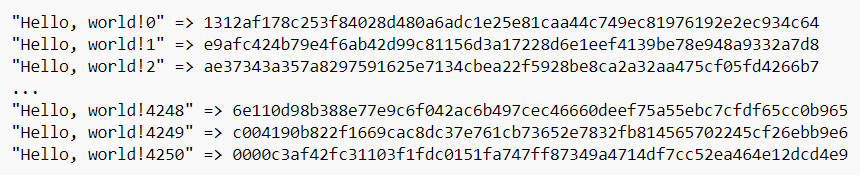
\includegraphics[width=0.9\linewidth]{Hash}
	\caption{Example of a proof of work (from bitwiki).}
	\label{fig:hash}
\end{figure}

\subsubsection{Mining a New Block}
The mining process is to solve the problem given by proof of work. At a given time, a node would gather transactions and form a block. To add this block to the block chain, the node has to solve the following problem:
\begin{align*}
&\text{Looking for a nonce $x$ such that: } Hash(s|x) < \text{target}\\
&s = s_1 | s_2 | s_3 | s_4 | s_5\\
&s_1 = \text{version}\\
&s_2 = \text{hash of previous block}\\
&s_3 = \text{hash of merkle root}\\
&s_4 = \text{timestamp }\\
&s_5 = \text{target}
\end{align*}
A block is composed of a block header and a block body. The block header is defined as $s|x$. Once a suitable nonce $x$ is found, the miner is can publish this block and add it to the block chain.
\subsection{General Procedure of Mining}
\begin{enumerate}
	\item Alice gathers the transactions and put them in a block (a block can contain approximately 4,000 transactions)
	\item Alice tries to solve the proof of work by finding a suitable nonce $x$
	\item If Alice is the first one to mine a new block, she may announce the block to the public and add it to the block chain
	\item If in the process of mining, a new block is mined by Bob. Alice abandons her block and restart step 1.
\end{enumerate}
\subsection{The Byzantine Generals' Problem}
A number of Byzantine Generals each has his own computer. They communicate through Internet to devise a plan to attack king's army. Only with a joint forces between the generals can they beat the king's army. However, several generals are spies deplored by the king. They would try to sabotage the proposed good plans. In this situation, the Byzantine General's Problem is given by how to agree upon a feasible plan to attack the king's army, given the condition that most of the generals (more than half in the case of bitcoin) are honest.


In the set up of bicoin, the Byzantine Generals' Problem is solved by the mining process at the cost of computational power (electricity). With the hard "inverse hash" step in the proof of work, the bitcoin system guarantees that no malicious user can double spend their bitcoins of forge a transaction, as will be shown in the next section.
\subsection{Double Spending and Forgery} 
Now Eve has ten bitcoins and she proposes transactions to both Bob and Alice to give them ten bitcoins each. In the meantime, there are two miners Charlie and Manuel.
\begin{enumerate}
	\item Eve announces a 10-bitcoin-transaction to  both Bob and Alice. (She only has 10 bitcoins left)
	\item Charlie first receives Eve's transaction to Alice, so he ignores Eve's transaction request to Bob.
	\item Due to delay of the Internet, Manuel first receives Eves transaction to Bob. So he ignores Eve's transaction request to Alice.
	\item Charlie and Manuel gather some transactions and both start to mine a block. 
	\item Without lose of generality, let's assume Manuel beats Charlie and solve the proof of work problem. Manuel happily add this new block to block chain. 
	\item Then Charlie would abandon his block. While gathering transactions for a new block, he would ignore Eve's transaction request because Eve's has already gave her remaining 10 bitcoins to Bob in the previous block mined by Manuel. 
\end{enumerate}

\section{References}
\begin{enumerate}
	\item The Mathematics Behind Bitcoin, Cyril Grunspan, \url{https://webusers.imj-prg.fr/~ricardo.perez-marco/blockchain/BitcoinP7.pdf}
	\item \url{https://en.bitcoinwiki.org/wiki}
\end{enumerate}
\end{document}